\documentclass{beamer}

\mode<presentation> {
\usetheme{Madrid}
%\usecolortheme{whale}
}
\RequirePackage{epsfig}
\usepackage[brazil]{babel}
\usepackage[utf8]{inputenc}
\usepackage{graphicx} % Allows including images
\usepackage{booktabs}
\usepackage{amsmath}% A
\usepackage{bm}
\usepackage{xcolor}
\usepackage{subfigure}
\usepackage{gensymb}
\usepackage{tikz}
\usepackage[document]{ragged2e}
\usetikzlibrary{shapes,backgrounds}
\graphicspath{{figures/}}


\newcommand{\nvec}{\mathbf{n}}
\newcommand{\xvec}{\mathbf{x}}
\newcommand{\vvec}{\mathbf{v}}
\newcommand{\mvec}{\mathbf{m}}
\newcommand{\uvec}{\mathbf{u}}
\newcommand{\fvec}{\mathbf{f}}
\newcommand{\zvec}{\mathbf{0}}
\newcommand{\xivec}{\boldmath \xi}

% Define block styles
\tikzstyle{block} = [rectangle, draw, fill=white, 
text width=6em, text centered, rounded corners, node distance=2cm, minimum height=2em]
\tikzstyle{line} = [draw, -latex]
\tikzstyle{cloud} = [draw, ellipse,fill=white, node distance=2cm,
minimum height=2em]


\title[Seminário]{Um exemplo simples de deslizamento em uma falha interna} % The short title appears at the bottom of every slide, the full title is only on the title page
% Macro com novos comandos

% pacotes
\usepackage{amssymb}
\usepackage{amsmath}
\usepackage[OT2,T1]{fontenc}
\DeclareSymbolFont{cyrletters}{OT2}{wncyr}{m}{n}
\DeclareMathSymbol{\Sha}{\mathalpha}{cyrletters}{"58}
\usepackage{xspace}
\usepackage{color}
\usepackage{cancel}
\usepackage{stackengine}
\usepackage{ulem}
\usepackage{enumerate}
\usepackage{mathtools}
\usepackage{tikz}
\usepackage{tikz-3dplot}
\usepackage{pgfplots}
\usepackage{xcolor}

% Criando comandos de correcao e comentarios
\newcommand{\rem}[1]{{\color{red} \sout{#1}}} % remover texto
\newcommand{\new}[1]{{\color{blue} #1}} % Incluir texto
\newcommand{\com}[1]{{\color{ao} #1}} % Incluir coment\'ario



% bibtex path
\newcommand{\mybib}{/home/daniel/Dropbox/latex/library}

%criando novas cores
\definecolor{amethyst}{rgb}{0.6, 0.4, 0.8}
\definecolor{ao}{rgb}{0.0, 0.5, 0.0}
\definecolor{tangerine}{rgb}{1.0, 0.6, 0.4}

% encurtando comandos
\newcommand{\tx}[1]{\text{#1}}
\newcommand{\tb}[1]{\textbf{#1}}
\newcommand{\ti}[1]{\textit{#1}}
%\newcommand{\Ref}[1]{(\ref{#1})}
\newcommand{\code}[1]{\begin{semiverbatim} #1 \end{semiverbatim}}
\newcommand{\mat}[1]{\mathbf{#1}}
\newcommand{\vc}[1]{\boldsymbol{#1}}


%letras gregas
\newcommand{\Aa}{\alpha}
\newcommand{\Bb}{\beta}
\newcommand{\ow}{\omega}
\newcommand{\Ow}{\Omega}
\newcommand{\sg}{\sigma}
\newcommand{\lb}{\lambda}
\newcommand{\lbx}{\lambda_x}
\newcommand{\vep}{\varepsilon}
\newcommand{\y}{\gamma}
\newcommand{\tht}{\theta}
\newcommand{\p}{\varphi}
\newcommand{\X}{\chi}
\newcommand{\phiiw}{\hat{\phi_i}}

\newcommand{\yi}{\gamma_i}
\newcommand{\Bbi}{\beta_i}

\newcommand{\DAa}{\Delta\alpha}
\newcommand{\DBb}{\Delta\beta}
\newcommand{\Drho}{\Delta\rho}
\newcommand{\Dsg}{\Delta\sigma}
\newcommand{\DT}{\Delta \tau}

%Hamiltoniana
\newcommand{\ham}{\mathcal{H}}
\newcommand{\co}{c_0}
\newcommand{\ce}{c_{\epsilon}}
\newcommand{\cdel}{c_{\delta}}
\newcommand{\nuj}{\nu_{j}}
\newcommand{\sj}{s_{j}}
% Deltas e deltas
\newcommand{\D}{\Delta}
\newcommand{\Dt}{\Delta t}
\newcommand{\Dw}{\Delta \ow}
\newcommand{\Dx}{\Delta x}
\newcommand{\Dy}{\Delta y}
\newcommand{\Dz}{\Delta z}
\newcommand{\Dr}{\Delta r}


% Caligraficas
\newcommand{\vTau}{\mathcal{T}}
\newcommand{\cC}{\mathcal{C}}
\newcommand{\cL}{\mathcal{L}}
\newcommand{\cO}{\mathcal{O}}
\newcommand{\cR}{{\cal R}}
\newcommand{\cH}{{\cal H}}
\newcommand{\FF}{\mathcal{F}}
\newcommand{\iFF}{\mathcal{F}^{-1}}

\newcommand{\cHm}[1][m]{\cH^{(#1)} }

% conjuntos
\newcommand{\F}{\mathbb{F}}
\newcommand{\R}{\mathbb{R}}
\newcommand{\I}{\mathbb{I}}
\newcommand{\C}{\mathbb{C}}
\newcommand{\Z}{\mathbb{Z}}
\newcommand{\N}{\mathbb{N}}

\newcommand{\fM}{\mathfrak{M}}

\newcommand{\M}[1][]{\mathbb{M}#1}
\newcommand{\MR}[1][\mn]{\M[#1](\R)}

%Vetores e matrizes
\newcommand{\ve}[1][i]{\boldsymbol{\hat{e}_{#1}}}

\newcommand{\matT}[1]{\mat{#1}^T}
\newcommand{\matH}[1]{\mat{#1}^{\ast}}

\newcommand{\mA}{\mat{A}}
\newcommand{\mAi}{\mA^{-1}}
\newcommand{\mAT}{\matT{A}}
\newcommand{\mAH}{\matH{A}}

\newcommand{\cofA}[2][\mA]{\Delta^{(#1)}_{#2}}
\newcommand{\cofAij}{\cofA{ij}}

\newcommand{\mB}{\mat{B}}
\newcommand{\mBi}{\mB^{-1}}
\newcommand{\mBT}{\matT{B}}
\newcommand{\mBH}{\matH{B}}

\newcommand{\mE}{\mat{E}}
\newcommand{\mH}{\mat{H}}
\newcommand{\mHX}{\mat{H}_{\X} }
\newcommand{\mHXb}{\bar{\mat{H}}_{\X} }
\newcommand{\mR}{\mat{R}}
\newcommand{\mC}{\mat{C}}
\newcommand{\mS}{\mat{S}}
\newcommand{\mX}{\mat{X}}
\newcommand{\mY}{\mat{Y}}
\newcommand{\mO}{\mat{0}}
\newcommand{\mI}{\mat{I}}
\newcommand{\mU}{\mat{U}}
\newcommand{\mV}{\mat{V}}
\newcommand{\mW}{\mat{W}}
\newcommand{\mL}{\mat{L}}
\newcommand{\mSg}{\mat{\Sigma}}
\newcommand{\hmL}{\hat{\mL}}

\newcommand{\mHm}[1][m]{\mH^{(#1)}}

\newcommand{\aij}[1][ij]{a_{#1}}
\newcommand{\bij}[1][ij]{b_{#1}}
\newcommand{\cij}[1][ij]{c_{#1}}

\newcommand{\maij}[2][ij]{\left[\aij[#1]\right]#2}
\newcommand{\mbij}[2][ij]{\left[\bij[#1]\right]#2}

\newcommand{\mn}{_{m \times n}}
\newcommand{\nn}{_{n \times n}}
\newcommand{\n}{_{n}}
\newcommand{\mxl}{_{m \times 1}}
\newcommand{\nxl}{_{n \times 1}}

\newcommand{\vi}{\,\hat{\vc{i}}}
\newcommand{\vj}{\,\hat{\vc{j}}}
\newcommand{\vk}{\,\hat{\vc{k}}}


\newcommand{\x}{\vc{x}}
\newcommand{\vu}{\vc{u}}
\newcommand{\hvu}{\hat{\vu}}
\newcommand{\vw}{\vc{w}}
\newcommand{\vx}{\vc{x}}
\newcommand{\vv}{\vc{V}}
\newcommand{\vh}{\vc{h}}
\newcommand{\vd}{\vc{d}}
\newcommand{\hvd}{\hat{\vc{d}}}
\newcommand{\vr}{\vc{r}}
\newcommand{\vf}{\vc{f}}
\newcommand{\vt}{\vc{\t}}
\newcommand{\vht}{\hat{\vc{t}}}
\newcommand{\vp}{\vc{p}}
\newcommand{\vy}{\vc{y}}
\newcommand{\vb}{\vc{b}}
\newcommand{\vhb}{\hat{\vc{b}}}
\newcommand{\va}{\vc{a}}
\newcommand{\vn}{\vc{n}}
\newcommand{\vhn}{\hat{\vc{n}}}
\newcommand{\vO}{\vc{0}}

\newcommand{\hvn}{\hat{\vn}}
\newcommand{\hvt}{\hat{\vt}}
\newcommand{\hp}{\hat{p}}
\newcommand{\hg}{\hat{g}}
\newcommand{\fw}{\skew{4.5}\hat{f}(\omega)}
\newcommand{\pxw}{\skew{4.5}\hat{P_x}}
\newcommand{\vwf}{\skew{4.5}\hat{V}}
\newcommand{\phixw}{\hat{\phi_x}}
\newcommand{\gw}{\skew{4.5}\hat{G}}
\newcommand{\Gw}{\skew{4.5}\hat{\mathcal{G}}}
\newcommand{\pw}{\skew{4.5}\hat{P}}
\newcommand{\qw}{\skew{4.5}\hat{q}(\vc{r},\ow)}
\newcommand{\ffw}{\vc{\skew{4.5}\hat{f}}(\vc{r},\ow)}

\newcommand{\vR}{\vc{R}}
\newcommand{\vF}{\vc{F}}
\newcommand{\vZ}{\vc{Z}}
\newcommand{\vY}{\vc{Y}}
\newcommand{\vW}{\vc{W}}
\newcommand{\vA}{\vc{A}}
\newcommand{\vB}{\vc{B}}
\newcommand{\vC}{\vc{C}}
\newcommand{\vD}{\vc{D}}
\newcommand{\vM}{\vc{M}}
\newcommand{\vG}{\vc{\Gamma}}
\newcommand{\vT}{\vc{\Theta}}
\newcommand{\vP}{\vc{\Phi}}


\newcommand{\m}{\vc{m}}
\newcommand{\tm}{\tilde{\vc{m}}}
\newcommand{\mz}{\m_0}
\newcommand{\mi}[1][]{\m_{i#1}}
\newcommand{\mj}{\m_j}
\newcommand{\mii}{\mi[+1]}
\newcommand{\dm}{\delta\m}
\newcommand{\dmest}{\delta m^{\est}}


\newcommand{\h}{\vc{h}}
\newcommand{\hz}{\h_0}
\newcommand{\hii}{\h_{i+1}}
\newcommand{\hi}{\h_i}
\newcommand{\hj}{\h_j}

% Funcoes
\newcommand{\ft}[1][]{f_{#1}(t)}
\newcommand{\gt}[1][]{g_{#1}(t)}
\newcommand{\hfw}[1][]{\hf_{#1}(\ow)}
\newcommand{\hhw}[1][]{\hh_{#1}(\ow)}
\newcommand{\fx}{f(x)}
\newcommand{\fxy}{f(x,y)}
\newcommand{\Pxy}{P(x,y)}
\newcommand{\Qxy}{Q(x,y)}
\newcommand{\fxyz}{f(x,y,z)}


\newcommand{\gx}{g(x)}
\newcommand{\gxy}{g(x,y)}
\newcommand{\yt}{y(t)}
\newcommand{\xt}{x(t)}
\newcommand{\yn}{y[n]}
\newcommand{\yk}{y_k}
\newcommand{\Yn}{Y_n}
\newcommand{\wN}[1][-nk]{w_N^{#1}}
\newcommand{\xn}{x[n]}
\newcommand{\mut}[1][]{\mu_{#1}(t)}
\newcommand{\mun}[1][]{\mu_{#1}[n]}
\newcommand{\hf}{\hat f}
\newcommand{\hx}{\hat x}
\newcommand{\hh}{\hat h}
\newcommand{\sgn}{\textrm{sgn} }
\newcommand{\sinc}{\textrm{sinc} }


\newcommand{\ep}[1][\ow t]{e^{i #1}}
\newcommand{\en}[1][\ow t]{e^{-i #1}}

\newcommand{\RtR}{\R \rightarrow \R}
\newcommand{\RtC}{\R \rightarrow \C}

% trigonometria
\newcommand{\sech}{\textrm{sech}}
\newcommand{\csch}{\textrm{csch}}


% Espa\c{c}os
\newcommand{\lp}[1][p]{\ell^#1}
\newcommand{\ld}{\lp[2]}

\newcommand{\Lp}[1][p]{L^#1}
\newcommand{\Ld}{\Lp[2]}

% Operadores
\renewcommand{\d}[2][]{\,\textrm{d}^{#1}#2}
\newcommand{\dx}[1][x]{\d{#1}}
\newcommand{\diiix}{\d[3]{\x}}
\newcommand{\diix}{\d[2]{\x}}
\newcommand{\dt}{\dx[t]}
\newcommand{\dr}{\dx[r]}
\newcommand{\dvr}{\dx[\vr]}
\newcommand{\ds}{\dx[s]}
\newcommand{\dtht}{\dx[\tht]}
\newcommand{\dtau}{\dx[\tau]}
\newcommand{\dy}{\dx[y]}
\newcommand{\dz}{\dx[z]}
\newcommand{\dw}{\dx[\ow]}
\newcommand{\dA}{\dx[A]}
\newcommand{\dV}{\dx[V]}
\newcommand{\dS}{\dx[S]}
\newcommand{\dvS}{\dx[\vc{S}]}

%\newcommand{\tr}{\textrm{tr}}
\newcommand{\posto}{\textrm{posto}}
\newcommand{\rank}{\textrm{rank}}
\newcommand{\nul}{\textrm{null}}
\newcommand{\im}{\textrm{Im}}
\newcommand{\re}{\textrm{Re}}


\newcommand{\dddtt}[1][]{\frac{\partial^2 #1}{\partial t^2}}
\newcommand{\dddxx}[1][]{\frac{\partial^2 #1}{\partial x^2}}
\newcommand{\dddxi}[1][]{\frac{\partial^2 #1}{\partial x_i^2}}
\newcommand{\dddzz}[1][]{\frac{\partial^2 #1}{\partial z^2}}
\newcommand{\dddyy}[1][]{\frac{\partial^2 #1}{\partial y^2}}
\newcommand{\ddd}[2][]{\frac{\partial^2 #1}{\partial #2^2}}
\newcommand{\dddc}[3][]{\frac{\partial^2 #1}{\partial #2 \partial #3}}

\newcommand{\ddy}[1][]{\frac{\partial #1}{\partial y}}
\newcommand{\ddi}[1][]{\frac{\partial #1}{\partial i}}
\newcommand{\ddz}[1][]{\frac{\partial #1}{\partial z}}
\newcommand{\ddx}[1][]{\frac{\partial #1}{\partial x}}
\newcommand{\ddt}[1][]{\frac{\partial #1}{\partial t}}
\newcommand{\dd}[2][]{\frac{\partial #1}{\partial #2}}

\newcommand{\DD}[2][]{\frac{\dx[#1]}{\dx[#2]}}
\newcommand{\DDn}[3][n]{\frac{\d[#1]#2}{\dx[#3]^{#1}}}

\newcommand{\DDx}[1][]{\frac{\dx[#1]}{\dx}}
\newcommand{\DDt}[1][]{\frac{\dx[#1]}{\dt}}
\newcommand{\DDDtt}[1][]{\frac{\dx[]^2#1}{\dt^2}}
\newcommand{\DDw}[1][]{\frac{\dx[#1]}{\dw}}


\newcommand{\lap}[1][]{\nabla^2_{#1}}
\newcommand{\Grad}[1][]{\nabla_{#1}}
\newcommand{\Div}[1][]{\nabla_{#1} \cdot }
\newcommand{\Rot}[1][]{\nabla_{#1} \times}

\newcommand{\dk}[1][]{\delta_{#1}}
\newcommand{\del}[1][t]{\delta\!\left(#1\right)}
\newcommand{\delc}[1][n]{\delta\left[#1\right]}

\newcommand{\intifif}{\int_{-\infty}^{\infty}}
\newcommand{\intOif}{\int_{0}^{\infty}}

\newcommand{\dint}{\displaystyle\int}

\newcommand{\sumifif}[1][n]{\sum_{#1=-\infty}^{\infty}}
\newcommand{\sumOif}[1][n]{\sum_{#1=0}^{\infty}}
\newcommand{\sumuif}[1][n]{\sum_{#1=1}^{\infty}}

\newcommand{\sumON}[1][k]{\sum_{#1=0}^{N-1}}

\newcommand{\norm}[2][]{\left\Vert#2\right\Vert_{#1}}
\newcommand{\mdl}[1]{\left|#1\right|}
\newcommand{\PI}[2]{\left\langle#1,#2\right\rangle}

\newcommand{\cchts}[1]{\left[#1\right]}
\newcommand{\Cchts}[1]{\left[\begin{array}#1 \end{array}\right]}
\newcommand{\prts}[1]{\left(#1\right)}
\newcommand{\chvs}[1]{\left\{#1\right\}}
\newcommand{\Chvs}[1]{\left\{\begin{array}#1 \end{array}\right\}}
\newcommand{\Sist}[1]{\left\{\begin{array}#1 \end{array}\right.}

\newcommand{\fft}[2][]{{\cal F}^{#1}\cchts{#2}}
\newcommand{\lplc}[2][]{{\cal L}^{#1}\cchts{#2}}
\newcommand{\hilb}[2][]{{\cal H}^{#1}\cchts{#2}}

% \newcommand{\mod}{\textrm{mod}}

%ondas elasticas
\newcommand{\kz}{k_z}
\newcommand{\ky}{k_y}
\newcommand{\kx}{k_x}

\newcommand{\kAa}{k_{\Aa}}
\newcommand{\kBa}{k_{\Bb}}

\newcommand{\vua}{\vu_{\Aa}}
\newcommand{\vub}{\vu_{\Bb}}

% Diferencas finitas
\newcommand{\uijn}[3][]{u_{i#1,j#2}^{n#3}}
\newcommand{\uin}[2][]{u_{i#1}^{n#2}}


\newcommand{\kij}[2][]{K_{i#1,j#2}}
\newcommand{\Pij}[3][t]{P_{i#2,j#3}(#1)}
\newcommand{\Vxij}[3][t]{V\!x_{i#2,j#3}(#1)}
\newcommand{\Vzij}[3][t]{V\!z_{i#2,j#3}(#1)}
\newcommand{\Vxijl}[3][]{V\!x_{i#1,j#2}^{l#3}(t)}
\newcommand{\Vzijl}[3][]{V\!z_{i#1,j#2}^{l#3}(t)}
\newcommand{\qij}[3][]{q_{i#2,j#3}}
\newcommand{\fxij}[2][]{fx_{i#1,j#2}}
\newcommand{\fzij}[2][]{fz_{i#1,j#2}}
\newcommand{\Rhoij}[2][]{\rho_{i#1,j#2}}
\newcommand{\Rhoxij}[2][]{\rho x_{i#1,j#2}}
\newcommand{\Rhozij}[2][]{\rho z_{i#1,j#2}}
\newcommand{\csi}{{\xi}_i}


\newcommand{\Pijl}[3][]{P_{i#1,j#2}^{l#3}}
\newcommand{\vxijl}[3][]{vx_{i#1,j#2}^{l#3}}
\newcommand{\vzijl}[3][]{vz_{i#1,j#2}^{l#3}}
\newcommand{\fxijl}[3][]{fx_{i#1,j#2}^{l#3}}
\newcommand{\fzijl}[3][]{fz_{i#1,j#2}^{l#3}}
\newcommand{\qijl}[3][]{q_{i#1,j#2}^{l#3}}


\newcommand{\Uijn}[3][]{U_{i#1,j#2}^{n#3}}
\newcommand{\Uin}[2][]{U_{i#1}^{n#2}}
\newcommand{\Un}[1][]{U^{n#1}}
\newcommand{\Ui}[1][]{U_{i#1}}

\newcommand{\odf}[2][2N]{\partial^{[#1]}_{#2}}

\newcommand{\Kij}[1][ij]{K^{#1} }
\newcommand{\hpij}[1][ij]{\hat{p}^{#1} }
\newcommand{\hqij}[1][ij]{\hat{q}^{#1} }
\newcommand{\hvxij}[1][ij]{\hat{v}_x^{#1} }
\newcommand{\hvzij}[1][ij]{\hat{v}_z^{#1} }
\newcommand{\hfxij}[1][ij]{\hat{f}_x^{#1} }
\newcommand{\hfzij}[1][ij]{\hat{f}_z^{#1} }
\newcommand{\rhoxij}[1][ij]{\rho_{(x)}^{#1} }
\newcommand{\rhozij}[1][ij]{\rho_{(z)}^{#1} }
\newcommand{\bxij}[1][ij]{b_{(x)}^{#1} }
\newcommand{\bzij}[1][ij]{b_{(z)}^{#1} }
\newcommand{\xixi}[1][i]{\xi_x^{#1}}
\newcommand{\xizj}[1][j]{\xi_z^{#1}}


% par\'agrafos especiais
\newcounter{ex}
\newcommand{\ex}[1][\theex]{\paragraph{Exerc\'icio #1}\stepcounter{ex}}

\newcounter{eg}
\newcommand{\eg}[1][\theeg]{\paragraph{Exemplo #1}\stepcounter{eg}}

\newcounter{qu}
\newcommand{\qu}[2][\thequ]{\paragraph{Quest\~ao #1 #2}\stepcounter{qu}}

% Transformada z
\newcommand{\az}{A(Z)}
\newcommand{\bz}{B(Z)}
\newcommand{\xz}{X(Z)}
\newcommand{\yz}{Y(Z)}
\newcommand{\fz}{F(Z)}
\newcommand{\wz}{W(Z)}
\newcommand{\pz}{P(Z)}

\newcommand{\baoz}{\bar A\left(\frac{1}{Z}\right)}
\newcommand{\bboz}{\bar B\left(\frac{1}{Z}\right)}
\newcommand{\bpoz}{\bar P\left(\frac{1}{Z}\right)}

% Micelanea

\newcommand{\vMb}{\bar{\vM}}
\newcommand{\vMd}{\dot{\vM}}

\newcommand{\xb}{\bar{x}}
\newcommand{\wb}{\bar{w}}
\newcommand{\wbm}{\bar{w}_m}

\newcommand{\vph}{\vc{\hat{p}}}
\newcommand{\vxi}{\vc{\xi}}

\newcommand{\matlab}{\textsc{Matlab}\xspace}
\newcommand{\latex}{\LaTeX\xspace}

\newcommand{\Pp}[1][(\x,\ow)]{P^+#1}
\newcommand{\Pn}[1][(\x,\ow)]{P^-#1}
\newcommand{\pp}[1][(\x,t)]{p^+#1}
\newcommand{\pn}[1][(\x,t)]{p^-#1}
\newcommand{\Pxw}[1][]{P_{#1}(\x,\ow)}
\newcommand{\Pxxw}[2][]{P(\x_{#1}|\x_{#2},\ow)}
\newcommand{\Gxxw}[3][]{G^{#1}(\x_{#2}|\x_{#3},\ow)}
\newcommand{\pxt}{p(\x,t)}
\newcommand{\QED}{\begin{flushright}
                   \textit{Q.E.D. ${\scriptstyle\blacksquare}$}
                  \end{flushright}
}

\newcommand{\ubar}[1]{\underset{\bar{}}{#1}}

\newcommand{\adj}{\textrm{adj}\, }

% \newcommand{\enumroman}[2][black]{\end{frame}

% \setbeamertemplate{enumerate item}{{\color{#1}\insertenumlabel}}
% #2
% \setbeamertemplate{enumerate items}[ball]
% \renewcommand{\theenumi}{\arabic{enumi}}}








\author{} % Your name
\institute[UFPA] % Your institution as it will appear on the bottom of every slide, may be shorthand to save space
{
	Professor: Jessé Costa\\
Universidade Federal do Pará \\ % Your institution for the title page
\medskip
 % Your email address
}
\date{\today} % Date

\setbeamercovered{transparent}

\AtBeginSection[]{
\begin{frame}
\frametitle{Sumário}
 \tableofcontents[currentsection]
\end{frame}
}



\begin{document}
 \begin{frame}
\begin{figure}[htb]
\centering

\includegraphics[width= 2cm, height= 2.5cm]{logo.jpg}
\end{figure}

\titlepage
\end{frame}

\begin{frame}{Um exemplo simples de deslizamento em uma falha interna}
		\justifying
\only<1>{Considere uma falha $\Sigma$ com vetor normal unit\'ario $\nu_{j}$ e tome $\xivec_{1}$, $\xivec_{2}$ e $\xivec_{3}$ como eixos coordenados na falha. 
Pressuponha que a falha $\Sigma$ est\'a situado no plano $\xivec_{3}=0$, de modo que as componentes do vetor normal $\nu_{1}$ e $\nu_{2}$ sejam nulos, $\nu_{1}= \nu_{2} =0$, pode-se alterar a equação abaixo
\begin{eqnarray}
\label{feq4}
f^{u}_{p}(\xvec',t) = -\int_{\Sigma}d\Sigma(\xivec) \, \left[u_{i}(\xivec,t) \right] \nu_j c_{ijpq}(\xivec) \frac{\partial}{\partial x'_{q}} \delta(\xvec' - \xivec) \, . \nonumber
\end{eqnarray} } 
\only<2>{Para o seguinte formato
\begin{eqnarray}
\label{feq8}
f^{u}_{p}(\xvec',t) = -\int_{\Sigma}d\xivec_{1}d\xivec_{2} \, \left[u_{1}(\xivec,t) \right] \nu_3 c_{13pq}(\xivec) \frac{\partial}{\partial x'_{q}} \delta(\xvec' - \xivec) \, . \nonumber
\end{eqnarray} 
Para um meio el\'astico isotr\'opico o tensor $c_{13pq}(\xivec)$ pode ser escrito da seguinte forma:
\begin{eqnarray*}
	\label{isotrop}
	c_{13pq} &=&  \lambda\delta_{13}\delta_{pq} + \mu(\delta_{1p}\delta_{3q} + \delta_{1q}\delta_{3p} )\, 
\end{eqnarray*}}
\end{frame}

\begin{frame}{Um exemplo simples de deslizamento em uma falha interna}
		\justifying
\visible<1->{Os \'unicos termos diferentes de zero da soma $\sum_{q}c_{13pq}$ s\~ao 
quando os \'indices $p=1$ e $q=3$, pela defini\c{c}\~ao da fun\c{c}\~ao delta e que devido a sim\'etria de $c_{13pq}=c_{13qp}$,
\begin{eqnarray*}
	\label{isotrop}
	c_{1313}(\xivec) &=&  \lambda\delta_{13}\delta_{13} + \mu(\delta_{11}\delta_{33} + \delta_{13}\delta_{31} ) \,\, = \,\, \mu(\xivec) \,\, = \,\, c_{1331}(\xivec) .
\end{eqnarray*}}
\only<2>{Desta forma, a equa\c{c}\~ao 
\begin{eqnarray}
\label{feq8}
f^{u}_{p}(\xvec',t) = -\int_{\Sigma}d\xivec_{1}d\xivec_{2} \, \left[u_{1}(\xivec,t) \right] \nu_3 c_{13pq}(\xivec) \frac{\partial}{\partial x'_{q}} \delta(\xvec' - \xivec) \, . \nonumber
\end{eqnarray} }
\only<3>{Para um meio isotr\'opico, mas ainda n\~ao homog\^eneo, \'e 
\begin{eqnarray}
\label{feq9_1}
f^{u}_{1}(\xvec',t) &=& -\int_{\Sigma}d\xivec_{1}d\xivec_{2} \,  \mu(\xivec)\left[u_{1}(\xivec,t) \right] \delta(x'_1 - \xivec_{1}) \delta(x'_2 - \xivec_{2}) \frac{\partial}{\partial x'_{3}} \delta(x_3') \, , \nonumber\\
f^{u}_{2}(\xvec',t) &=& 0\, ,\nonumber\\
\label{feq9_2}
f^{u}_{3}(\xvec',t) &=& -\int_{\Sigma}d\xivec_{1}d\xivec_{2} \, \mu(\xivec)\left[u_{1}(\xivec,t) \right] \frac{\partial}{\partial x'_{1}} \delta(x_1' - \xivec_1) \delta(x'_2 - \xivec_{2}) \delta(x'_3)\, . \nonumber
\label{feq9_3}
\end{eqnarray}
}

\end{frame}


\begin{frame}{Um exemplo simples de deslizamento em uma falha interna}
		\justifying
A partir deste momento, serão avaliadas as equações abaixo  para determinar dois modelos de fontes 
s\'ismicas produzidos pelo deslizamento de uma falha interna em uma \'unica dire\c{c}\~ao:
sistema de bin\'ario \'unico e sistema de for\c{c}as \'unicas, respectivamente.
\begin{eqnarray}
\label{feq9_1}
f^{u}_{1}(\xvec',t) &=& -\int_{\Sigma}d\xivec_{1}d\xivec_{2} \,  \mu(\xivec)\left[u_{1}(\xivec,t) \right] \delta(x'_1 - \xivec_{1}) \delta(x'_2 - \xivec_{2}) \frac{\partial}{\partial x'_{3}} \delta(x_3') \, , \nonumber\\
f^{u}_{3}(\xvec',t) &=& -\int_{\Sigma}d\xivec_{1}d\xivec_{2} \, \mu(\xivec)\left[u_{1}(\xivec,t) \right] \frac{\partial}{\partial x'_{1}} \delta(x_1' - \xivec_1) \delta(x'_2 - \xivec_{2}) \delta(x'_3)\, . \nonumber
\label{feq9_3}
\end{eqnarray}
\end{frame}

\begin{frame}{Sistema de bin\'arios \'unicos}
		\justifying
\visible<1->{Considerando que a for\c{c}a $f^{u}_{1}(\xvec',t)$ esteja atuando na dire\c{c}\~ao $\pm x'_{1}$ com o bra\c{c}o ao longo da dire\c{c}\~ao $x'_{2}$ e o momento angular ao longo da dire\c{c}\~ao $x'_{3}$ 
e distribu\'idas sobre a falha $\Sigma$. }
\only<1>{\\Assim, a equa\c{c}\~ao
\begin{eqnarray}
\label{feq9_1}
f^{u}_{1}(\xvec',t) &=& -\int_{\Sigma}d\xivec_{1}d\xivec_{2} \,  \mu(\xivec)\left[u_{1}(\xivec,t) \right] \delta(x'_1 - \xivec_{1}) \delta(x'_2 - \xivec_{2}) \frac{\partial}{\partial x'_{3}} \delta(x_3') \, , \nonumber
\end{eqnarray}
}
\visible<2->{\\Fica desta forma \begin{eqnarray*}
		f^{u}_{1}(\xvec',t) &=& - \left\{  \int_{\Sigma}d\xivec_{1}d\xivec_{2} \, \mu(\xivec)\left[u_{1}(\xivec,t) \right]  \delta(x'_1 - \xivec_{1}) \delta(x'_2 - \xivec_{2}) \right\} \frac{\partial}{\partial x'_{3}} \delta(x_3') \, ,
\end{eqnarray*}}
\only<3>{Utilizando a propriedade de filtragem da fun\c{c}\~ao delta de Kronecker
\begin{eqnarray*}
	\label{feq11}
	\int_{\Sigma}d\xivec_{1}d\xivec_{2} \, \mu(\xivec)\left[u_{1}(\xivec,t) \right] \delta(x'_1 - \xivec_{1}) \delta(x'_2 - \xivec_{2}) =  \mu(\xvec')\left[u_{1}(\xvec',t) \right] \, ,
\end{eqnarray*}}
\visible<4>{Reduz equa\c{c}\~ao acima para, agora com coordenadas fora da regi\~ao de falha,
	\begin{eqnarray}
	\label{feq10}
	f^{u}_{1}(\xvec',t) &=& - \mu(\xvec')\left[u_{1}(\xvec',t) \right] \frac{\partial}{\partial x'_{3}} \delta(x_3') \, \nonumber .     
	\end{eqnarray}}

\end{frame}

\begin{frame}{Sistema de bin\'arios \'unicos}
		\justifying
O momento total sobre o eixo $x'_2$ \'e,  
usando equa\c{c}\~ao 
\begin{eqnarray}
\label{feq6}
\int_{\Omega}d\Omega(\xvec') \, (\xvec' - \xvec'_{0}) \wedge f^{u}_{p}(\xvec',t) = \zvec \, , \nonumber
\end{eqnarray} 
Tem-se 
\small{\begin{eqnarray*}
	\int_{\Omega}d\Omega\, \epsilon_{231} x'_{3} f^{u}_{1}(\xvec',t) \\ =  -\int_{x'_{1}}dx'_{1}\int_{x'_{2}}dx'_{2}\int_{x'_{3}}dx'_{3} \, x'_{3}\mu(x'_{1},x'_{2},x'_{3}) \left[ u_{1}(x'_{1},x'_{2},x'_{2},t)\right] \frac{\partial }{\partial x'_{3}} \delta(x'_3)  \,& ,\\
	= -\int_{x'_{1}}dx'_{1}\int_{x'_{2}}dx'_{2} \left\{ \int_{x'_{3}}dx'_{3} \, x'_{3} \frac{\partial }{\partial x'_{3}} \delta(x'_3)  \right\} \mu(x'_{1},x'_{2},x'_{3}) \left[ u_{1}(x'_{1},x'_{2},x'_{3},t)\right] &  \, ,
\end{eqnarray*} }
\end{frame}

\begin{frame}{Sistema de bin\'arios \'unicos}
		\justifying
Fazendo a integração por parte no termo entre colchetes, 
	\begin{eqnarray*}
		\int_{x'_{3}}dx'_{3} \, x'_{3} \frac{\partial }{\partial x'_{3}} \delta(x'_3)  &=& x'_{3}\delta(x'_{3}) - \int_{x'_3} dx'_3\,\delta(x'_3) \, ,
	\end{eqnarray*} 
 Isso significa que estamos no plano de falha $\Sigma$, ent\~ao as coordenadas 
$x'_1$ e $x'_2$ s\~ao agora $\xivec_1$ e $\xivec_2$, respectivamente, que leva \`a
\begin{eqnarray*}
	\int_{\Omega}d\Omega\, \epsilon_{231} x'_{3} f^{u}_{1}(\xvec',t) &=& \int_{\xivec_1}d\xivec_1 \int_{\xivec_2}d\xivec_2 \,  \mu(\xivec_{1},\xivec_{2},0) \left[ u_{1}(\xivec_{1},\xivec_{2},0,t)\right] \, ,\\
	&=& \int_{\Sigma}d\Sigma \, \mu(\xivec) \left[ u_{1}(\xivec,t)\right]   \, ,    
\end{eqnarray*}
\end{frame}

\begin{frame}{Sistema de binários únicos}
		\justifying
Multiplicando o resultado acima pela \'area da falha, que definimos como $A = \int_{\Sigma} d\Sigma$ e  
assumido que a regi\~ao de falha \'e homog\^enea, ou seja, $\mu$ \'e uma constante, ent\~ao obtemos 
\begin{eqnarray} 
\label{momtotal1}
\int_{\Omega}d\Omega\, x'_{3} f^{u}_{1}(\xvec',t) &=&  \mu  \left\{ \frac{ \int_{\Sigma}d\Sigma \,  \left[ u_{1}(\xivec,t)\right]}{A} \right\} A  \,\,  = \,\, \mu \bar{u}(t) A \, ,  \nonumber
\end{eqnarray} 
onde $\bar{u}(t)$ \'e definido como a m\'edia do deslizamento na falha,
\begin{eqnarray*}  
	\bar{u}(t) &=& \frac{ \int_{\Sigma}d\Sigma \,  \left[ u_{1}(\xivec,t)\right]}{A} \, .
\end{eqnarray*}  
\end{frame}

\begin{frame}{Sistemas de forças únicas}
		\justifying
\only<1>{A partir da equação
\begin{eqnarray}
f^{u}_{3}(\xvec',t) &=& -\int_{\Sigma}d\xivec_{1}d\xivec_{2} \, \mu(\xivec)\left[u_{1}(\xivec,t) \right] \frac{\partial}{\partial x'_{1}} \delta(x_1' - \xivec_1) \delta(x'_2 - \xivec_{2}) \delta(x'_3)\, . \nonumber
\label{feq9_3}
\end{eqnarray}
representando um sistema de forças únicas.}
\visible<2->{Reescrevendo:
\begin{eqnarray*}  
	\label{feq11}
	f^{u}_{3}(\xvec',t) &=& -  \frac{\partial}{\partial x'_{1}} \left\{ \int_{\Sigma}d\xivec_{1}d\xivec_{2} \, \mu(\xivec)\left[u_{1}(\xivec,t) \right] \delta(x_1' - \xivec_1) \delta(x'_2 - \xivec_{2}) \right\} \delta(x'_3)\, .    
\end{eqnarray*}}
\only<3>{Utilizando a propriedade de filtragem da fun\c{c}\~ao delta de Kronecker, 
	\begin{eqnarray*}
		\label{feq11}
		\int_{\Sigma}d\xivec_{1}d\xivec_{2} \, \mu(\xivec)\left[u_{1}(\xivec,t) \right] \delta(x'_1 - \xivec_{1}) \delta(x'_2 - \xivec_{2}) =  \mu(\xvec')\left[u_{1}(\xvec',t) \right] \, ,
\end{eqnarray*}}
\visible<4->{Reduzindo-a para
\begin{eqnarray*}
	f^{u}_{3}(\xvec',t) &=&  -\frac{\partial }{\partial x'_{1}} \left\{ \mu(\xvec') \left[ u_{1}(\xvec',t)\right]\right\} \delta(x'_3)  \, .
\end{eqnarray*}}

\end{frame}

\begin{frame}{Sistemas de forças únicas}
		\justifying
	\only<1>{Para obter o momento total vamos substituir o resultado anterior na equação
	\begin{eqnarray}
	\label{feq6}
	\int_{\Omega}d\Omega(\xvec') \, (\xvec' - \xvec'_{0}) \wedge f^{u}_{p}(\xvec',t) = \zvec \, , \nonumber
	\end{eqnarray}  }
\visible<2->{Tem-se
\begin{eqnarray*}
	\int_{\Omega}d\Omega\, \epsilon_{213} x'_{1} f^{u}_{1}(\xvec',t)\\ =  \int_{x'_{1}}dx'_{1}\int_{x'_{2}}dx'_{2}\int_{x'_{3}}dx'_{3} \, x'_{1}  \frac{\partial }{\partial x'_{1}} \left\{ \mu(x'_{1},x'_{2},x'_{3}) \left[ u_{1}(x'_{1},x'_{2},x'_{2},t)\right] \right\} \delta(x'_3)  \, ,\\
	= \int_{x'_{1}}dx'_{1}\int_{x'_{2}}dx'_{2} \left\{ \int_{x'_{3}}dx'_{3} \, \delta(x'_3)  \right\} x'_{1} \frac{\partial }{\partial x'_{1}} \left\{ \mu(x'_{1},x'_{2},x'_{3}) \left[ u_{1}(x'_{1},x'_{2},x'_{3},t)\right] \right\} \, ,
\end{eqnarray*} 
}
\end{frame}

\begin{frame}{Sistemas de forças únicas}
	\small
		\justifying
\visible<1->{Onde a integral entre cochetes \'e igual a $1$ quando $x'_3 = 0$ o que novamente nos leva ao plano de falha $\Sigma$, ou seja,
\begin{eqnarray*}
	\int_{\Omega}d\Omega\, \epsilon_{213} x'_{1} f^{u}_{1}(\xvec',t) &=& 
	\int_{\xivec_{2}} d\xivec_{2} \left\{ \int_{\xivec_{1}} d\xivec_{1} \xivec_{1} \frac{\partial }{\partial \xivec_{1}} \left\{ \mu(\xivec_{1},\xivec_{2},0) \left[ u_{1}(\xivec_{1},\xivec_{2},0,t)\right] \right\}  \right\}  \, 
\end{eqnarray*}	}
\visible<2->{Utilizando a integração por partes
\begin{eqnarray*}
	\int_{\xivec_{1}} d\xivec_{1} \xivec_{1} \frac{\partial }{\partial \xivec_{1}} \left\{ \mu(\xivec_{1},\xivec_{2},0) \left[ u_{1}(\xivec_{1},\xivec_{2},0,t)\right] \right\} &=& \xivec_{1} \mu(\xivec_{1},\xivec_{2},0) \left[ u_{1}(\xivec_{1},\xivec_{2},0,t)\right] \\ 
	&-& \int_{\xivec_{1}} d\xivec_{1} \mu(\xivec_{1},\xivec_{2},0) \left[ u_{1}(\xivec_{1},\xivec_{2},0,t)\right]  \, ,
\end{eqnarray*}
}

\end{frame}

\begin{frame}{Sistemas de forças únicas}
		\justifying
Usando uma superf\'icie de falha $\Sigma$ definida para ter $\left[ u_{1}(\xivec_{1},\xivec_{2},0,t)\right] = 0$ em torno de seu per\'imetro, obtemos
\begin{eqnarray*}
	\int_{\Omega}d\Omega\, \epsilon_{213} x'_{1} f^{u}_{1}(\xvec',t) &=& -\int_{\xivec_1}d\xivec_1 \int_{\xivec_2}d\xivec_2 \,  \mu(\xivec_{1},\xivec_{2},0) \left[ u_{1}(\xivec_{1},\xivec_{2},0,t)\right] \, ,\\
	&=& - \int_{\Sigma}d\Sigma \, \mu(\xivec) \left[ u_{1}(\xivec,t)\right]   \, ,    
\end{eqnarray*}	
multiplicando o resultado acima pela \'area da falha $A = \int_{\Sigma} d\Sigma$ 
e tomamos $\mu$ constante, ent\~ao
\begin{eqnarray} 
\label{momtotal2}
\int_{\Omega}d\Omega\, x'_{3} f^{u}_{1}(\xvec',t) &=&  -\mu  \left\{ \frac{ \int_{\Sigma}d\Sigma \,  \left[ u_{1}(\xivec,t)\right]}{A} \right\} A  \,\,  = \,\, -\mu \bar{u}(t) A \, ,  \nonumber
\end{eqnarray} 
onde $\bar{u}(t)$ \'e a m\'edia do deslizamento na falha,
\begin{eqnarray*}  
	\bar{u}(t) &=& \frac{ \int_{\Sigma}d\Sigma \,  \left[ u_{1}(\xivec,t)\right]}{A} \, .
\end{eqnarray*} 
\end{frame}

\begin{frame}{Sistemas binários duplos}
		\justifying
No entanto, não há uma relação um para um entre as forças equivalentes e o deslizamento de
uma dada falha. Mostraremos isso  obtendo:
\begin{itemize}
	\item Uma densidade de bin\'ario duplo;
	\item uma densidade de bin\'ario \'unico ou for\c{c}a \'unica, assim recorre-se ao teorema da representa\c{c}\~ao
	\begin{eqnarray*}
		\label{feq11}
		\int_{\Sigma}d\xivec_{1}d\xivec_{2} \, \mu(\xivec)\left[u_{1}(\xivec,t) \right] \delta(x'_1 - \xivec_{1}) \delta(x'_2 - \xivec_{2}) =  \mu(\xvec')\left[u_{1}(\xvec',t) \right] \, , \nonumber
	\end{eqnarray*}
para descrever a falha, $\xivec_3=0$, com deslizamento na dire\c{c}\~ao $\xivec_1$, 
\small{\begin{eqnarray*}
	u_{n}(\xvec,t) = \int_{-\infty }^{+\infty}d\tau\int_{\Sigma}d\Sigma(\xivec) 
	\, \left[ u_{1}(\xivec,\tau)\right] \nu_{3}c_{13pq}(\xivec) \frac{\partial}{\partial \xi_q} G_{np}(\xvec,t-\tau;\xivec,0) \,& \nonumber \\
	 =    \int_{-\infty }^{+\infty}d\tau\int_{\Sigma}d\Sigma(\xivec)  
	\, \left[ u_{1}(\xivec,\tau)\right] \nu_{3} \left\{ \sum_{p=1}^{3} \sum_{q=1}^{3}  c_{13pq}(\xivec) \frac{\partial}{\partial \xi_q} G_{np}(\xvec,t-\tau;\xivec,0) \right\}  \, , &
\end{eqnarray*}}
\end{itemize}
\end{frame}

\begin{frame}{Sistemas binários duplos}
	\small
	Avaliando a soma em $p$ 
	\begin{eqnarray*}
		\sum_{p=1}^{3} \sum_{q=1}^{3} c_{13pq}(\xivec) \frac{\partial G_{np} }{\partial \xi_q}  = \sum_{q=1}^{3}\left\{ c_{131q}(\xivec) \frac{\partial  G_{n1}}{\partial \xi_q} +  c_{132q}(\xivec) \frac{\partial G_{n2}}{\partial \xi_q}  + c_{133q}(\xivec) \frac{\partial G_{n3}}{\partial \xi_q}  \right\} \, ,
	\end{eqnarray*}
Ap\'os usar a sim\'etria $c_{1313} = c_{1331} = \mu$, encontramos
\begin{eqnarray}
\label{feq12}
u_{n}(\xvec,t) &=& \int_{-\infty }^{+\infty}d\tau\int_{\Sigma}d\Sigma(\xivec) 
\, \left[ u_{1}(\xivec,\tau)\right] \nu_{3} \mu(\xivec) \frac{\partial }{\partial \xi_3}G_{n1}(\xvec,t-\tau;\xivec,0) \, \nonumber\\
&+&\int_{-\infty }^{+\infty}d\tau\int_{\Sigma}d\Sigma(\xivec) 
\, \left[ u_{1}(\xivec,\tau)\right] \nu_{3} \mu(\xivec) \frac{\partial}{\partial \xi_1}G_{n3}(\xvec,t-\tau;\xivec,0)  \, ,  \nonumber            
\end{eqnarray}
	
\end{frame}
\begin{frame}{Sistemas binários duplos}
		\justifying
A primeira derivada da equação anterior \'e o limite 
	da aproxima\c{c}\~ao de ponto central de primeira ordem da expans\~ao da s\'erie de Taylor de pontos vizinhos 
	ao plano de falha, $\pm\varepsilon\hat{\xivec_3}$,
	\begin{eqnarray*}   
		\frac{\partial G_{n1}}{\partial \xi_3}  =  \lim_{\varepsilon \rightarrow 0} \, \frac{G_{n1}(\xvec,t-\tau;\xivec + \varepsilon \hat{\xivec_3},0) - G_{n1}(\xvec,t-\tau;\xivec - \varepsilon \hat{\xivec_3} ,0) }{2\varepsilon} \, ,            
	\end{eqnarray*}
A segundo derivada 
 \'e tamb\'em o limite 
da aproxima\c{c}\~ao de ponto central de primeira ordem da expans\~ao da s\'erie de Taylor de pontos vizinhos 
ao plano de falha, $\pm\varepsilon\hat{\xivec_1}$,
\begin{eqnarray*}   
	\frac{\partial G_{n3}}{\partial \xi_1}  =  \lim_{\varepsilon \rightarrow 0} \, \frac{G_{n3}(\xvec,t-\tau;\xivec + \varepsilon \hat{\xivec_1},0) - G_{n3}(\xvec,t-\tau;\xivec - \varepsilon \hat{\xivec_1} ,0) }{2\varepsilon} \, ,            
\end{eqnarray*}
\end{frame}

\begin{frame}{Sistemas binários duplos}
		\justifying
	Estes dois últimos resultados que encontramos
	representam separadamente a distribuição de dois sistemas de binários únicos em oposição ao
	resultado que encontramos a partir das equações
	\begin{eqnarray}
	\label{feq9_1}
	f^{u}_{1}(\xvec',t) &=& -\int_{\Sigma}d\xivec_{1}d\xivec_{2} \,  \mu(\xivec)\left[u_{1}(\xivec,t) \right] \delta(x'_1 - \xivec_{1}) \delta(x'_2 - \xivec_{2}) \frac{\partial}{\partial x'_{3}} \delta(x_3') \, , \nonumber\\
	f^{u}_{2}(\xvec',t) &=& 0\, ,\nonumber\\
	\label{feq9_2}
	f^{u}_{3}(\xvec',t) &=& -\int_{\Sigma}d\xivec_{1}d\xivec_{2} \, \mu(\xivec)\left[u_{1}(\xivec,t) \right] \frac{\partial}{\partial x'_{1}} \delta(x_1' - \xivec_1) \delta(x'_2 - \xivec_{2}) \delta(x'_3)\, . \nonumber
	\label{feq9_3}
	\end{eqnarray}
	onde se obteve uma distribuição de
	binário único mais uma distribuição de força única.
	\only<1>{Integrando por partes $\partial G_{n1}/\partial \xi_{3}$ ou $\partial G_{n3}/\partial \xi_{1}$ de
	\begin{eqnarray}
	\label{feq12}
	u_{n}(\xvec,t) &=& \int_{-\infty }^{+\infty}d\tau\int_{\Sigma}d\Sigma(\xivec) 
	\, \left[ u_{1}(\xivec,\tau)\right] \nu_{3} \mu(\xivec) \frac{\partial }{\partial \xi_3}G_{n1}(\xvec,t-\tau;\xivec,0) \, \nonumber\\
	&+&\int_{-\infty }^{+\infty}d\tau\int_{\Sigma}d\Sigma(\xivec) 
	\, \left[ u_{1}(\xivec,\tau)\right] \nu_{3} \mu(\xivec) \frac{\partial}{\partial \xi_1}G_{n3}(\xvec,t-\tau;\xivec,0)  \, ,  \nonumber            
	\end{eqnarray}}
\visible<2->{\\Tem-se
\begin{eqnarray*}
	\int_{\Sigma}d\Sigma(\xivec)\, \frac{\partial G_{n3} }{\partial \xi_1} &=&  
	\, \left[ u_{1}(\xivec,\tau)\right] G_{n3}   -  \int_{\Sigma}d\Sigma(\xivec)\, \left[ \frac{\partial u_{1}(\xivec,\tau) }{\partial \xi_1} \right]G_{n3}  \, ,              
\end{eqnarray*}}
\end{frame}

\begin{frame}{Sistemas binários duplos}
		\justifying
Definindo novamente que no per\'imetro/bordas da falha $\Sigma$ o campo $\left[ u_{1}(\xivec,t)\right] = 0$, ent\~ao temos
\begin{eqnarray}
\label{feq13}
u_{n}(\xvec,t) &=& \int_{-\infty }^{+\infty}d\tau\int_{\Sigma}d\Sigma(\xivec) 
\, \mu(\xivec) \left[ u_{1}(\xivec,\tau)\right]\frac{\partial }{\partial \xi_3} G_{n1}(\xvec,t-\tau;\xivec,0)   \, \nonumber \\
&- & \int_{-\infty }^{+\infty}d\tau\int_{\Sigma}d\Sigma(\xivec) 
\, \mu(\xivec) \left[ \frac{\partial u_{1}(\xivec,\tau) }{\partial \xi_1} \right]G_{n3}(\xvec,t-\tau;\xivec,0)\, , \nonumber
\end{eqnarray}
\end{frame}

\begin{frame}{Sistemas de binários como fontes pontuais}
	\justifying
Considere agora que falha $\Sigma$ esteja localizada a uma grande dist\^ancia em rela\c{c}\~ao a 
posi\c{c}\~ao de observa\c{c}\~ao $\xvec$, de modo que as \'unicas ondas observadas s\~ao aquelas 
com comprimentos de onda muito maiores do que as dimens\~oes lineares da falha.
\begin{eqnarray*}
	\left[ u_{1}(\xi_1,\xi_2,t)\right] &=&  \bar{u}A\delta(\xi_1) \delta(\xi_2) H(t)\, ,
\end{eqnarray*}
\only<1>{substituindo-a nas componentes $f^{u}_{1}(\xvec',t)$ e $f^{u}_{3}(\xvec',t)$ das equa\c{c}\~oes
\begin{eqnarray}
\label{feq9_1}
f^{u}_{1}(\xvec',t) &=& -\int_{\Sigma}d\xivec_{1}d\xivec_{2} \, \mu(\xivec)\left[u_{1}(\xivec,t) \right] \delta(x'_1 - \xivec_{1}) \delta(x'_2 - \xivec_{2}) \frac{\partial}{\partial x'_{3}} \delta(x_3') \,\nonumber , \\
f^{u}_{2}(\xvec',t) &=& 0\, \nonumber,\\
\label{feq9_2}
f^{u}_{3}(\xvec',t) &=& -\int_{\Sigma}d\xivec_{1}d\xivec_{2} \, \mu(\xivec)\left[u_{1}(\xivec,t) \right] \frac{\partial}{\partial x'_{1}} \delta(x_1' - \xivec_1) \delta(x'_2 - \xivec_{2}) \delta(x'_3)\, .\nonumber
\label{feq9_3}
\end{eqnarray}}
\visible<2->{Tem-se 
\begin{eqnarray}
\label{feq14_1}
f^{u}_{1}(\xvec',t) &=& -M_{0}\delta(x'_1) \delta(x'_2) \frac{\partial}{\partial x'_{3}} \delta(x_3') H(t) \,\nonumber , \\
f^{u}_{2}(\xvec',t) &=& 0\, \nonumber,\\
\label{feq14_2}
f^{u}_{3}(\xvec',t) &=& -M_{0} \frac{\partial}{\partial x'_{1}} \delta(x_1') \delta(x'_2) \delta(x'_3) H(t)\,\nonumber ,
\label{feq14_3}
\end{eqnarray}
onde $M_{0}$ \'e definido como o momento s\'ismico,
\begin{eqnarray}
\label{feq15}
M_{0} = \mu \bar{u} A\,\nonumber ,
\end{eqnarray}
}

	
	
	
\end{frame}

\begin{frame}
	\begin{figure}[htb]
		\centering
		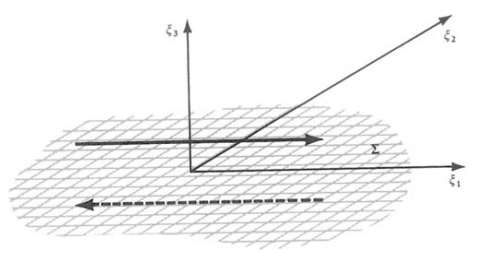
\includegraphics[width= 8cm, height= 8cm]{superficie}
	\end{figure}
\end{frame}

\begin{frame}
	\begin{equation}
	\begin{matrix}
	f_1(\vc{\eta},\tau) &=& -M_0\delta(\eta_1)\delta(\eta_2)\frac{\partial}{\partial \eta_3}\delta(\eta_3)H(\tau) \nonumber \\
	f_2(\vc{\eta},\tau)& =& 0 \nonumber \\
	f_3(\vc{\eta},\tau) &=& -M_0\frac{\partial}{\partial \eta_1}\delta(\eta_1)\delta(\eta_2)\delta(\eta_3)H(\tau)
	\end{matrix}
	\end{equation}
	$$M_0 =  \mu \bar{u}A = \mu \times \text{deslizamento médio} \times \text{área de falha} $$
	$$\text{log} M_0 = 1.5 M_w + 16.1 $$
\end{frame}



\begin{frame}
	\begin{figure}[htb]
		\centering
		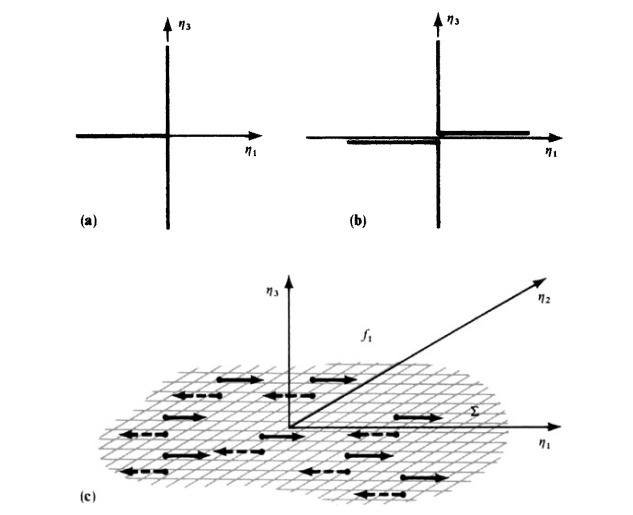
\includegraphics[width= 8cm, height= 8cm]{diagramas}
	\end{figure}
\end{frame}

\begin{frame}
	\begin{figure}[htb]
		\centering
		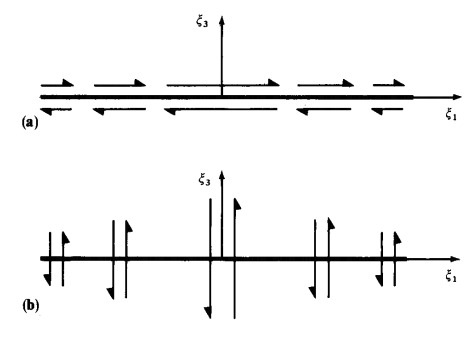
\includegraphics[width= 8cm, height= 8cm]{distribuicao}
	\end{figure}
\end{frame}

\begin{frame}
	\begin{figure}[htb]
		\centering
		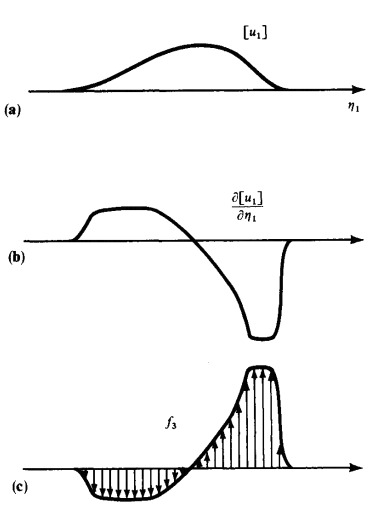
\includegraphics[width= 8cm, height= 8cm]{terceira}
	\end{figure}
\end{frame}

\begin{frame}
	\begin{figure}[htb]
		\centering
		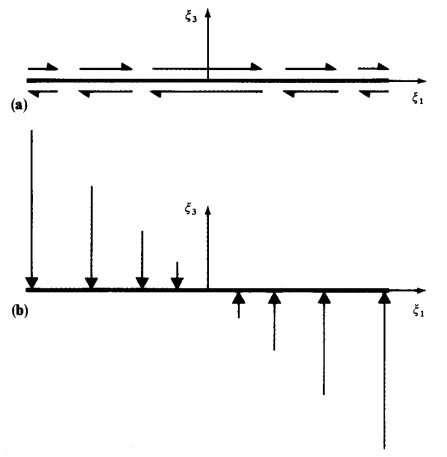
\includegraphics[width= 8cm, height= 8cm]{forca}
	\end{figure}
\end{frame}



\end{document}